\documentclass{article}
\usepackage{amsmath}
\usepackage{siunitx}
\usepackage{xcolor}
\usepackage{hyperref}
\usepackage{graphicx}
\usepackage{listings}
\lstset{language=Python,%
	basicstyle=\footnotesize\ttfamily,stringstyle=\color{red!40!black},%
	commentstyle=\color{violet!95!black}\textsf,%
	keywordstyle=\color{green!30!black}, morekeywords={as},%
	tabsize=3,breaklines=true,postbreak=\mbox{\textcolor{red}{$\hookrightarrow$}\space}, showstringspaces=false,%
	backgroundcolor = \color{black!3!white}}
\usepackage[a4paper, left=2cm, right=2cm, top=2cm, bottom=2cm]{geometry}

\author{Marco Codato}
\title{Notes}

\begin{document}
\maketitle

\section{Introduction}

\paragraph{What I have done yet (chronological order):}
\begin{itemize}
	\item The script can save the bkg masked spectrum in a new file, copying the original header too.
	\item Write a python script that opens a given \texttt{.fits} file, automatically detects the astronomical sources and removes them, providing the spectrum of the background (bkg) only.
\end{itemize}

\paragraph{What I am doing/going to do soon:}
\begin{itemize}
	\item It would be nice to include in the new header more information, e.g.\ when the script was runt, which rows were deleted and so on\dots
	\item Develop a more solid and qualitative framework wrt what reported below.
\end{itemize}




\paragraph{Next steps (likely):}
\begin{itemize}
	\item Test the script with more frames to check the robustness.
	\item Decide wether integrate the bkg over the slit position or not.
	\item ISSUE: if we want to retrieve the sky brightness (insted of the flux only) we have to consider that observations are carried on a portion of the sky delimited by the CCD spatial size (namely the ``height'') and the size of the slit. The problem is that the slit size is quite uncertain and heavily affects the precision of the computation.
	\item Understand how to disentangle the natural sky emission and the contribution from artificial illumination.
\end{itemize}

\paragraph{Future major steps (likely):}
\begin{itemize}
	\item Decide how to model the various contributions to the bkg spectrum, in particular LED lights have very different types of spectra.
	\item Fit the data to obtain the weights of the various sources of the bkg.
	\item Develope a convenient strategy to find correlation between the results of the fit and the observation condition.
\end{itemize}

\section{Background spectrum extraction}

\subsection{Automatic detection}
\begin{itemize}
	\item Integrate over all the wavelenghts by summing the data in the dispersion direction. In this way a can synthetically see the flux along the spatial direction, regardless the source (i.e.\ continuum or line).
	\item Detect the peaks the integrated flux using the function \href{https://docs.scipy.org/doc/scipy/reference/generated/scipy.signal.find_peaks.html}{\texttt{scipy.signal.find\_peaks}}. This function finds the local maxima of an 1D signal.
	
	On the current data it was convenient to filter the detected peak to have a \href{https://en.wikipedia.org/wiki/Topographic_prominence}{prominence} (in this case $\sim$ height from the background) higher than 0.5\% the highest peak on the signal. This helped to neglect local maxima due to spatial noise fluctuations.
	
	\item Measure the width of each peak with \href{https://docs.scipy.org/doc/scipy/reference/generated/scipy.signal.peak_widths.html#scipy.signal.peak_widths}{\texttt{scipy.signal.peak\_widths}}. This function is designed to work with noisy signal and several maxima and minima, instead of just some maxima above a flat background. I set the option \texttt{rel\_height=0.5} to measure the FWHM of each peack instead of the width at the base, which turned to be not very solid for the data we had.
	
	\item Mask the regions around the peaks. After some testing, the best strated (with the data available) is to remove a region of width $ 5\times$ FWHM around each peak.
	
	Note if peak profile fits a gaussian appriximation (i.e.\ sharp peaks and/or high SNR and/ord profile intrisically gaussian) then 5 FWHM correspond span to $5.89\sigma$ from the maximum, when the flux is dimmed by a factor \num{e-8}.
	
	Such an high span is required as many sources have not gaussian profiles and in particular might present bright wings wrt the gaussian prediction (e.g.\ galaxies have a bright nearly gaussian core plus faint but extended spiral arms).
	
	\item Extract the data of the background as those outside the region of the peaks. These are the areas that will be used for the analysis.
\end{itemize}
Note that due to the variety of luminosity profiles of astronomical sources it is not very efficient to develope a qualitative approach to compute the best width. This empirical treatment is good enough (if it will prove to be solid with more data though).


\subsection{Preliminary results}
Here the results with the two frames available.

\paragraph{NGC2392 (2006/ima\_010).} The Eskimo Nebula. There is a sharp peak with strong wings. Probably another very faint source is present in the field. The script does recognize both the signals and removes them.

\begin{figure}[h!]
	\begin{minipage}{.49\textwidth}
		\centering
		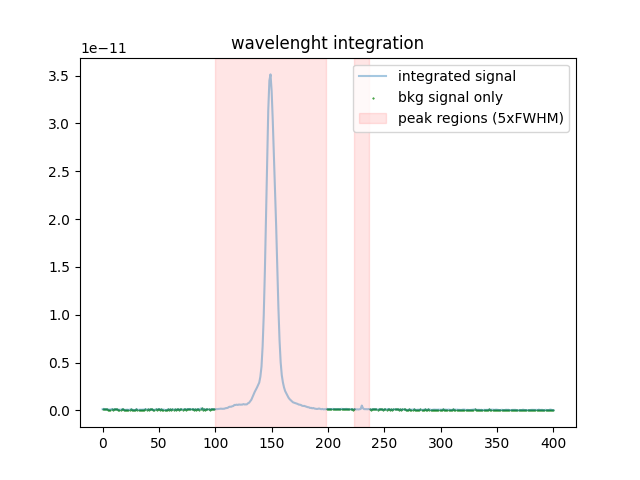
\includegraphics[width=\textwidth]{10_1}
	\end{minipage}
\hfill
	\begin{minipage}{.49\textwidth}
	\centering
	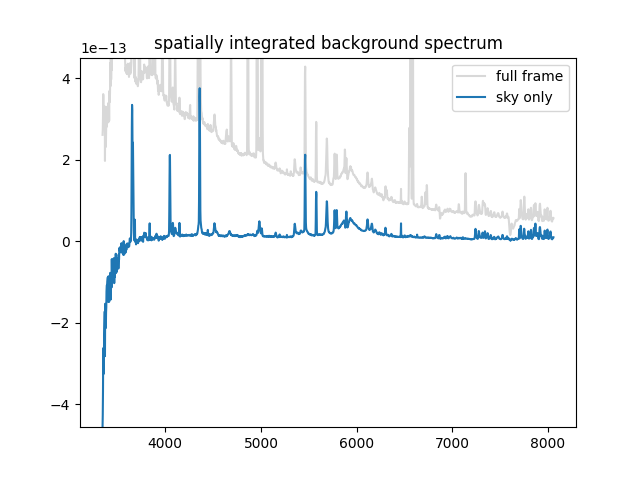
\includegraphics[width=\textwidth]{10_2}
\end{minipage}
\end{figure}
\begin{figure}[h!]
	\centering
	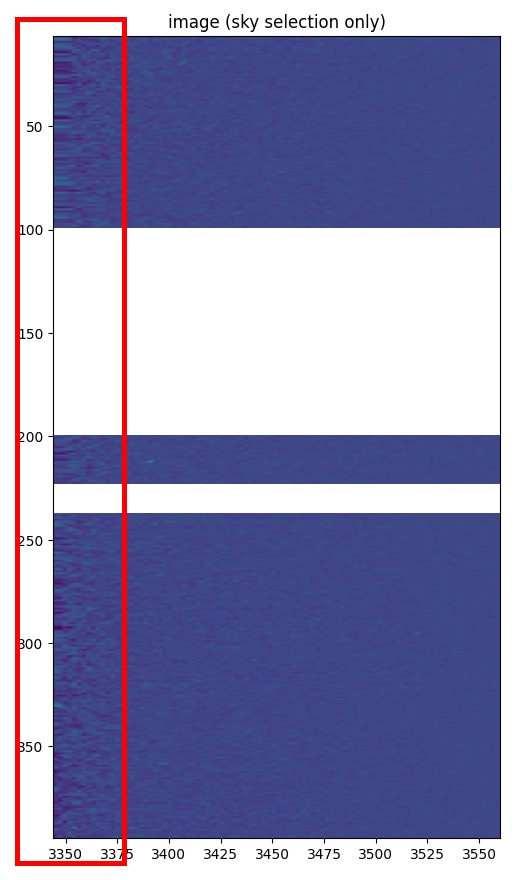
\includegraphics[width=.35\textwidth, angle=90]{10_det}
\end{figure}
We integrate over all the position along the slit where we no astronomical sources/signals are present. Then we plot it against the wavelenght to obtain the spectrum of the background (atmospheric emission + light pollution).

In the removal they comes out negative fluxes in the bluer hand of the spectrum. We realize that the wavelenght range in this frame begins at $\sim\SI{3344}{\angstrom}$ which considerable as UV radiation. It is not so surprising to find inaccurate results at those extreme wavelenghts.


\paragraph{Ark564 (2006/ima\_015).} In this case the sources along the slit seems to be several but the script seems to be able to manage all of them.
\begin{figure}[h!]
	\begin{minipage}{.49\textwidth}
		\centering
		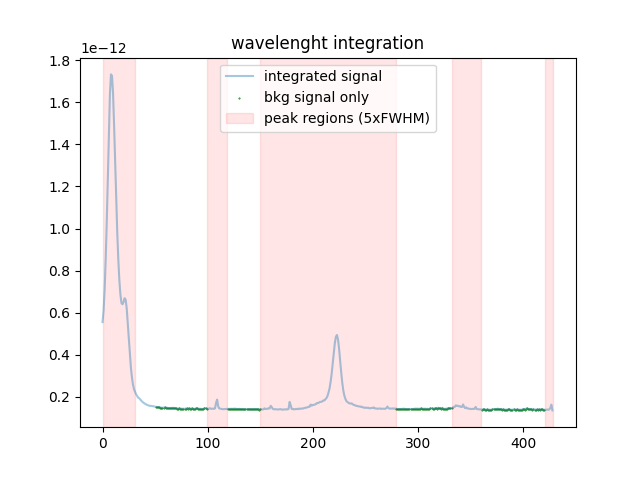
\includegraphics[width=\textwidth]{15_1}
	\end{minipage}
	\hfill
	\begin{minipage}{.49\textwidth}
		\centering
		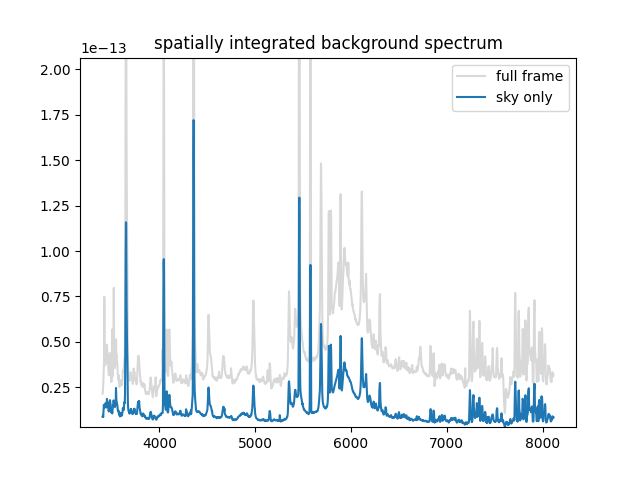
\includegraphics[width=\textwidth]{15_2}
	\end{minipage}
\end{figure}
In this case the spectrum of the background do not seem to present any issue.

\subsection{Comments on the first results}
\paragraph{Wavelenght limitations.} It would be convenient to set a wavelenght treshold for the analized data. Wavelenghts outside the spectrograph+telescope working range may led to biased measurements.

\paragraph{Frame limitations(?)} I wonder wether the whole CCD area is suitable for collecting data or it would be better/necessary to neglect some specific regions, both in the spatial and dispersion directions.

\textcolor{red}{What about the lines ``\texttt{CCDSEC}'' and ``\texttt{BIASSEC}'' in the header of the frames?}

\newpage
\section{Appendix: Python source code}
The code I am using.
\lstinputlisting[language=Python]{../pippo.py}

\end{document}

